%! TEX root = main.tex

\subsection{Imagine...}
\begin{frame}\frametitle{\insertsubsection}

You are Andrew Wiles.

You worked on a marvelous proof on a conjecture for \(6\) years, and finally publish it.

Two months later, a critical flaw was discovered, and your work is voided. \emoji{frowning-face}

If only that computers can verify Mathematical proofs...

\end{frame}



\subsection{Formalise? What?}
\begin{frame}\frametitle{\insertsubsection}

We can \textbf{formalise} proofs. Informally, it means to

\begin{definition}
  Rewrite Mathematical proofs in a machine-understandable language.
\end{definition}

The language I used is the \texttt{Lean 4} language + its Mathematics library \texttt{Mathlib 4}.

\end{frame}



\subsection{Formalise? What? \emoji{eyes}}
\begin{frame}\frametitle{\insertsubsection}

\begin{block}{Transitivity}
  Let \(P, Q, R\) be \textit{logical} statements. If \(P \implies Q\) and \(Q \implies R\), then \(P \implies R\).
\end{block}

\begin{proof}
  Suppose \(P\) holds. Then by \(P \implies Q\), we know that \(Q\) holds. And since \(Q \implies R\), we know that \(R\) holds. Hence, \(P\) implies \(R\).
\end{proof}

\begin{figure}
  \centering
  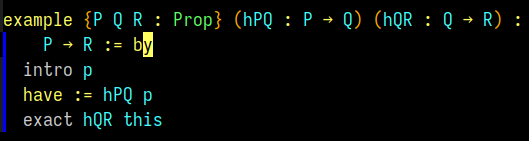
\includegraphics[scale=0.6]{images/demo.png}
\end{figure}

\end{frame}



% \subsection{Formalise? Why?}
% \begin{frame}\frametitle{\insertsubsection}
%
% \begin{enumerate}
%   \item Now: Build up mathematical library
%   \item Now/Future: Verify more complicated proofs (in real time!)
%   \item Fun!
% \end{enumerate}
%
% \end{frame}



\subsection{Formalise what? (My project)}
\begin{frame}\frametitle{\insertsubsection}

For my 3\textsuperscript{rd} year project, I formalised a extremal combinatorics result in 2021 by Ben Green, under the supervision of Damiano Testa.

The resulting project is original work building on top of the \texttt{Lean 4 + Mathlib 4} libraries.

To my knowledge, this is the \textbf{best} result of this type formalised in any theorem prover.

\end{frame}
